\documentclass{article}
\usepackage[utf8]{inputenc}
\usepackage{graphicx,amsmath,subcaption,float}

\title{Ph20.7: Linear and Non-linear Regression: The Hubble plot using Type-1a Supernovae}
\author{Sophie Li}
\date{March 2019}

\begin{document}
\maketitle
\section{Initial Plots}
\begin{figure}[H]
    \centering
    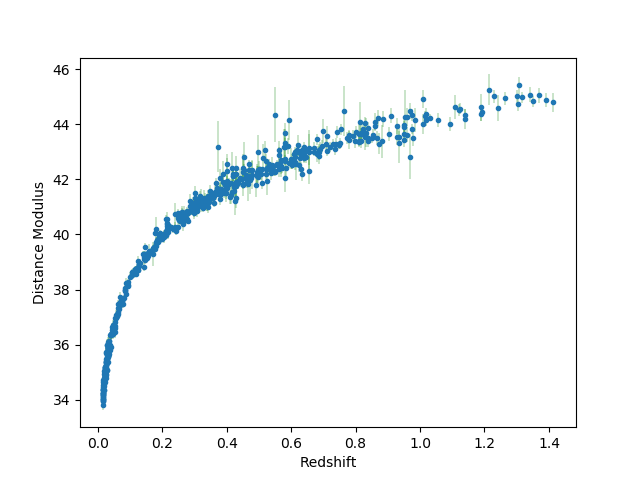
\includegraphics[width = \textwidth]{Images/redshiftdm.png}
    \caption{Red shift vs. Distance Modulus}
    \label{fig:redshiftdm}
\end{figure}

\begin{figure}[H]
    \centering
    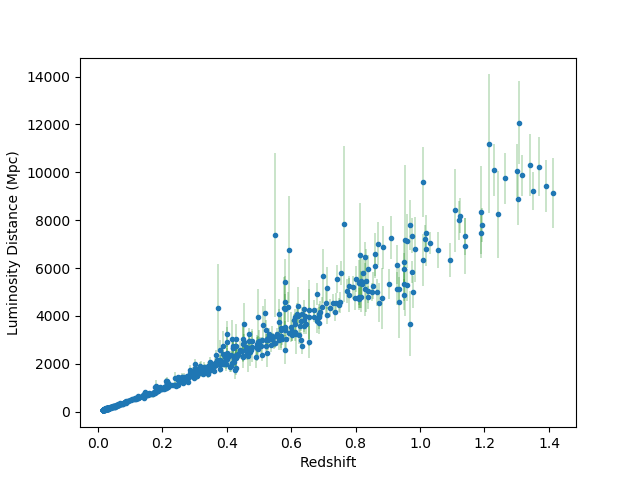
\includegraphics[width = \textwidth]{Images/redshiftld.png}
    \caption{Red shift vs. Luminosity Distance}
    \label{fig:redshiftld}
\end{figure}

\section{Linear Hubble's Law}
\begin{figure}[H]
    \centering
    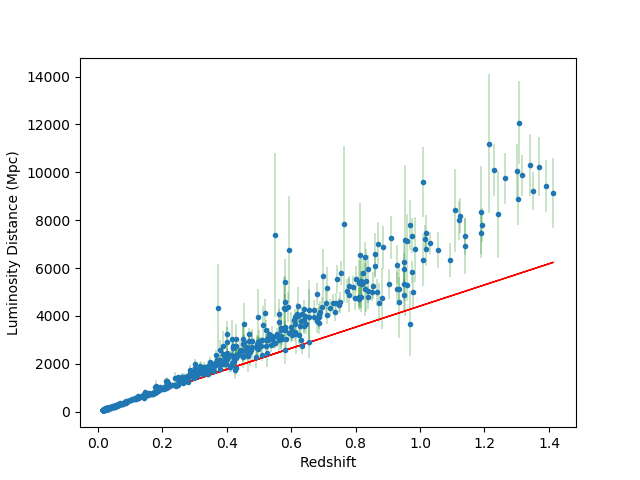
\includegraphics[width = \textwidth]{Images/linfit.png}
    \caption{Linear Hubble's Law to Red shift vs. Luminosity Distance}
    \label{fig:linfit}
\end{figure}
For the linear Hubble's Law we got a $H_0 = 67.19$. 

\section{Non-linear Hubble's Law}
\begin{figure}[H]
    \centering
    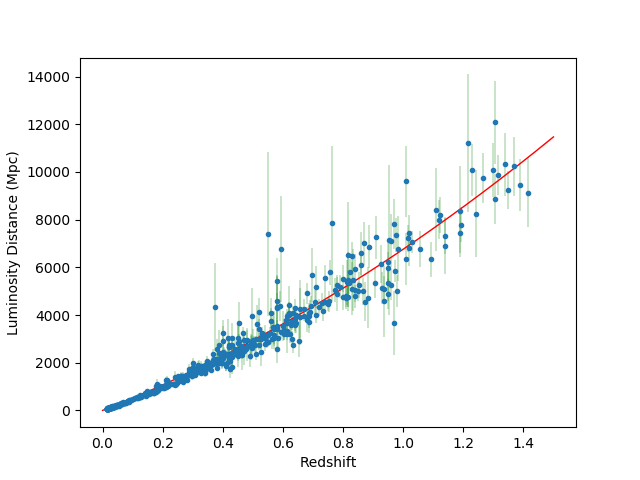
\includegraphics[width = \textwidth]{Images/nonlinfit.png}
    \caption{Non-linear Hubble's Law to Red shift vs. Luminosity Distance}
    \label{fig:nonlinfit}
\end{figure}
For the non-linear Hubble's law we got $H_0 = 60.19$ and $q = 0.2861$
\section{FLRW Metric Expression}
\begin{figure}[H]
    \centering
    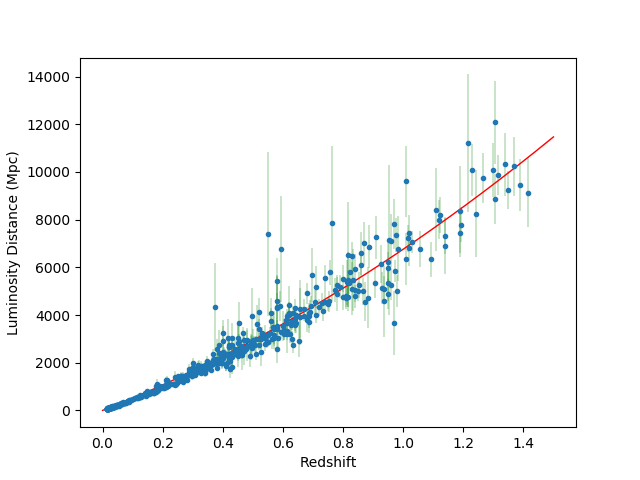
\includegraphics[width = \textwidth]{Images/nonlinfit.png}
    \caption{Non-linear Hubble's Law to Red shift vs. Luminosity Distance}
    \label{fig:nonlinfit}
\end{figure}
For the FLRW metric experession for luminosity distance we got $H_0 = 62.12$ and $\Omega_M = 0.3679$. From the fit we have that the value of $\Omega_M$  has $\sigma^2 = 0.0021706$. This means that for $\Omega_\Lambda= 1 - \Omega_M$, this means that for $\Omega_\Lambda$ there is a statistical significance of 13.57. This is a very high value for statistical significance and thus strongly suggests that $\Omega_\Lambda > 0$ and thus that the universe is expanding.
\end{document}